\documentclass[10pt]{ctexbeamer}
\usepackage[utf8]{inputenc}
\usepackage{xeCJK}
\usepackage{graphicx}
\usepackage{mathtools}
\usepackage{utopia} %font utopia imported
\usepackage{hyperref}
\usetheme{CambridgeUS}
\usecolortheme{dolphin}


% 南邮VI手册给出了南邮指定的颜色代码,
\definecolor{cstd}{cmyk}{100,90,0,0}
\definecolor{cblue}{cmyk}{80,30,0,0}
\definecolor{green}{cmyk}{60,0,100,0}
\definecolor{cyellow}{cmyk}{0,20,100,0}
\definecolor{cblack}{cmyk}{0,0,0,100}
\definecolor{cgrey}{cmyk}{0,0,0,60}
\definecolor{clightgrey}{cmyk}{0,0,0,30}

% 使用转换工具https://www.qtccolor.com/secaiku/tool/convert?m=cmyk将颜色转换为RGB,
% 这样可以获得较好的显示效果
\definecolor{rstd}{RGB}{2,55,139}
\definecolor{rblue}{RGB}{9,142,202}
\definecolor{rgreen}{RGB}{121,180,28}
\definecolor{ryellow}{RGB}{253,203,0}
\definecolor{rblack}{RGB}{26,23,27}
\definecolor{rgrey}{RGB}{134,135,137}
\definecolor{rlightgrey}{RGB}{197,198,199}

%使用南邮的配色设置内容
\setbeamercolor*{palette primary}{bg=rgreen}
\setbeamercolor*{palette secondary}{bg=rblue, fg = white}
\setbeamercolor*{palette tertiary}{bg=rstd, fg = white}
\setbeamercolor*{titlelike}{fg=rstd}
\setbeamercolor*{title}{bg=rstd, fg = white}
\setbeamercolor*{item}{fg=rstd}
\setbeamercolor*{caption name}{fg=rstd}
\usefonttheme{professionalfonts}

% 增加参考文献引用支持
\usepackage[backend=biber,autolang=hyphen,style=gb7714-2015,
gbtype=true,gbalign=gb7714-2015,
doi=false,url=false,isbn=false]{biblatex}
% 引入参考文献数据库
\addbibresource[location=local]{reference.bib}

%增加指导老师
\newcommand{\theadvisor}{}
\newcommand{\advisor}[1]{
  \renewcommand{\theadvisor}{#1}
}

%------------------------------------------------------------
%使用校训作为logo
\logo{
\includegraphics[width=.2\textwidth]{pic/njupt.motto.pdf}}

% 设置段落首行缩进
\setlength\parindent{20pt}
\setlength\parskip{0pt}

%设置标题页
\setbeamertemplate{title page}{%

\includegraphics[height=1.2cm]{pic/njupt.logo_full.pdf}\par
\vspace*{10pt}
\centering
  \songti\selectfont
    {%
    \usebeamerfont{title}
        \inserttitle
    }\par
    {%
    \usebeamerfont{subtitle}
        \insertsubtitle
    }\par\medskip
    {%
    \color{rstd}
        \rule{\linewidth}{1pt}
    }\par\medskip
    
    {%
    \usebeamercolor[fg]{author}
    \usebeamerfont{author}
      汇报人:\insertauthor\par\smallskip
      指导老师:\theadvisor\par\smallskip
    }
    \vspace*{10pt}
    {%
    \usebeamercolor[fg]{institute}
    \usebeamerfont{institute}
        \insertinstitute
    }\par\medskip
    \vspace*{10pt}
    {%
    \usebeamercolor[fg]{date}
    \usebeamerfont{date}
        \insertdate
    }\par
}

%------------------------------------------------------------
%This block of commands puts the table of contents at the 
%beginning of each section and highlights the current section:
% \AtBeginSection[]
% {
%  \begin{frame}
%    \frametitle{Contents}
%    \tableofcontents[currentsection]
%  \end{frame}
% }
\AtBeginSection[]{
  \setbeamertemplate{background} 
  {
    \centering
    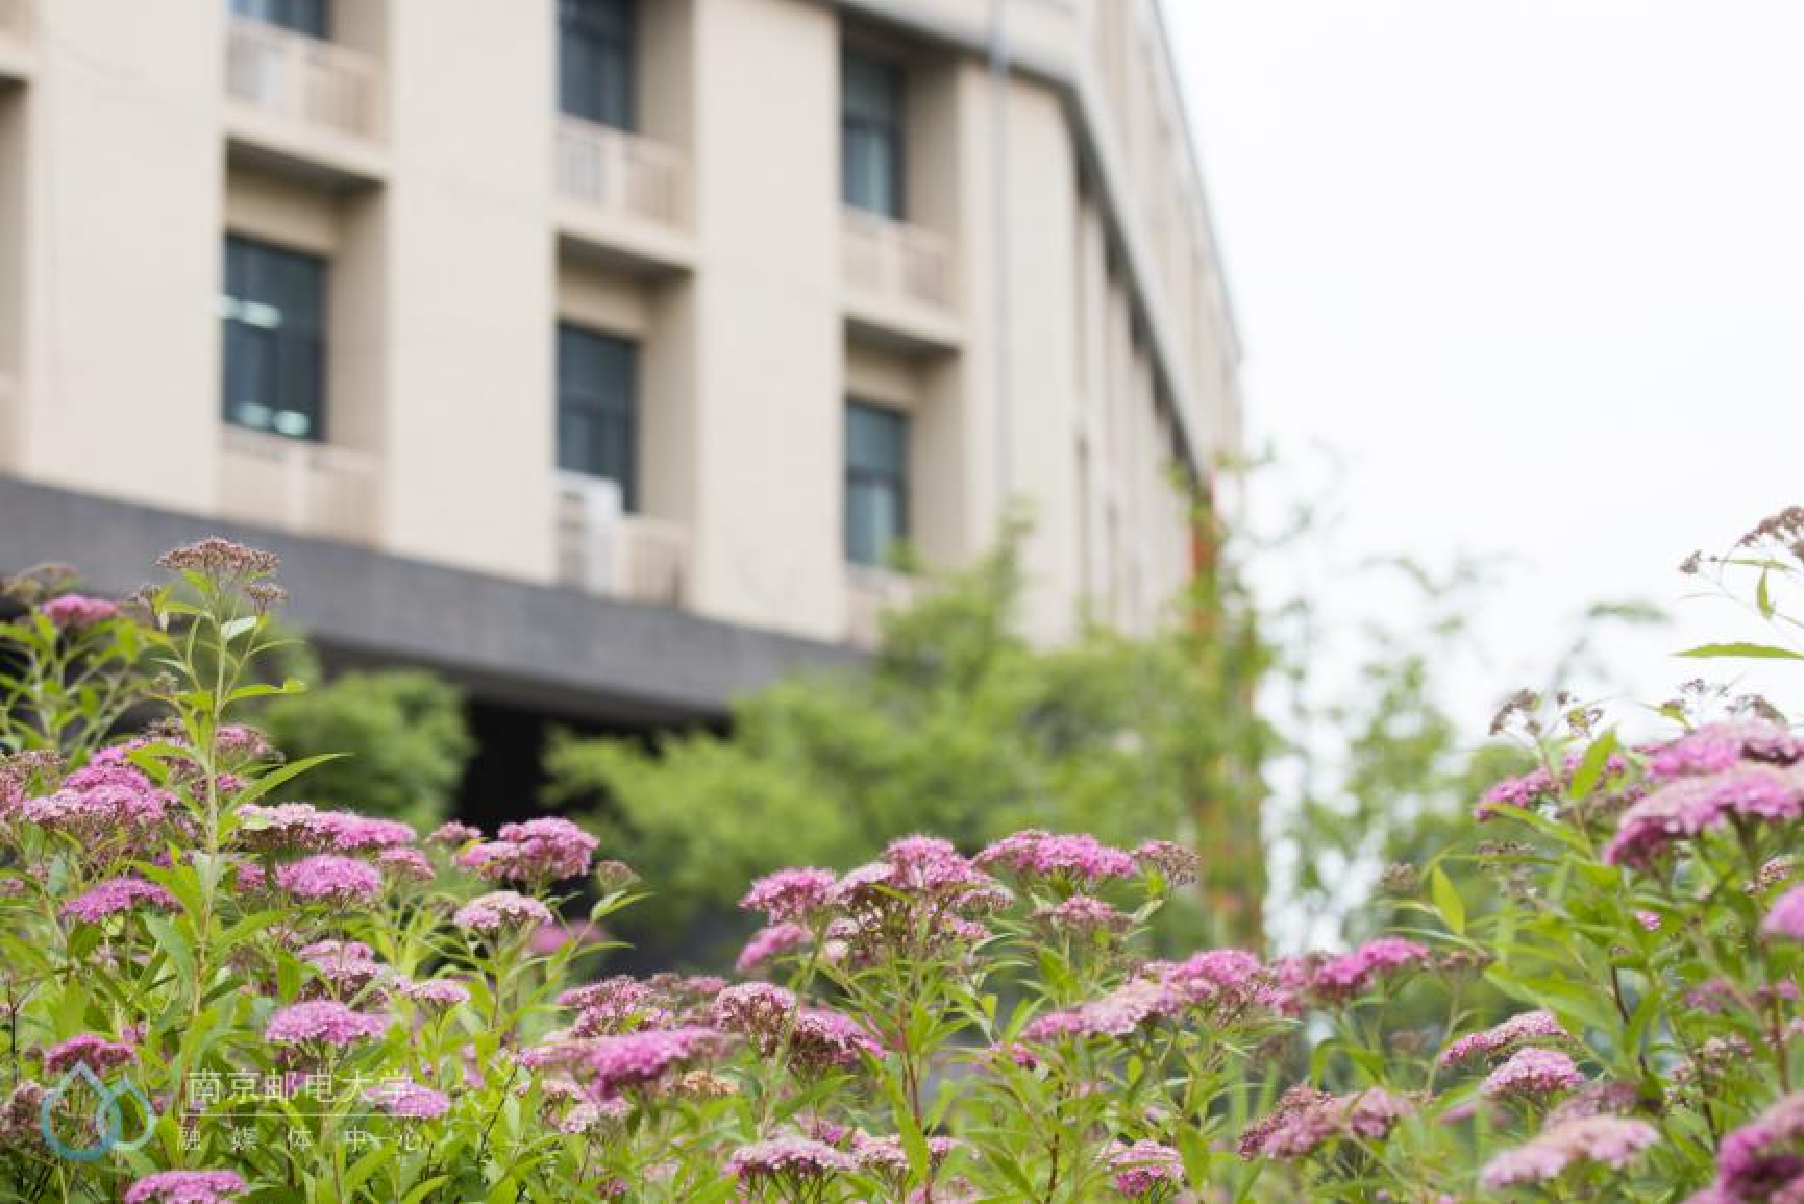
\includegraphics[trim=0 100 0 0,height=\paperheight,angle=0]{pic/njupt.flower.pdf}
  }
  \begin{frame}
  \vfill
  \centering
  \begin{beamercolorbox}[sep=8pt,center,shadow=true,rounded=true]{title}
    \usebeamerfont{title}\insertsectionhead\par%
  \end{beamercolorbox}
  \vfill
  \end{frame}
  \setbeamertemplate{background}{}
}

%------------------------------------------------------
%正式内容从此处开始
%------------------------------------------------------

\title[南京邮电大学]{控制理论的三个月与三十年}
\subtitle{Three Months and Tirty Years of Control}
\author[李倩茹]{李倩茹、 沈梦辰}
\advisor{丕艾谛}
\institute[自动化学院、人工智能学院]{
南京邮电大学

自动化学院、人工智能学院
}
\date[南京 \today]{南京 \today}

%------------------------------------------------------------

%可以为不同的部分设置不同的字体
% %设置不同部分的字体,注意不同设备中安装的字体会不同
% \renewcommand{\normalfont}{\fangsong}
% \setbeamerfont{title}{family=\heiti,series=\bfseries}
% %帧标题字体
% \setbeamerfont{frametitle}{family=\heiti,series=\bfseries}
% %帧子标题字体
% \setbeamerfont{framesubtitle}{family=\kaishu,series=\bfseries}
% \setbeamerfont{footline}{family=\kaishu,size=\tiny}

%设置字号大小
\setbeamerfont{title}{size=\Large}
\setbeamerfont{subtitle}{size=\small}
\setbeamerfont{author}{size=\small}
\setbeamerfont{date}{size=\tiny}
\setbeamerfont{institute}{size=\small}


\begin{document}

%创建标题页
\frame{\titlepage}

%创建目录页
\setbeamertemplate{background} 
{
    \raggedright
    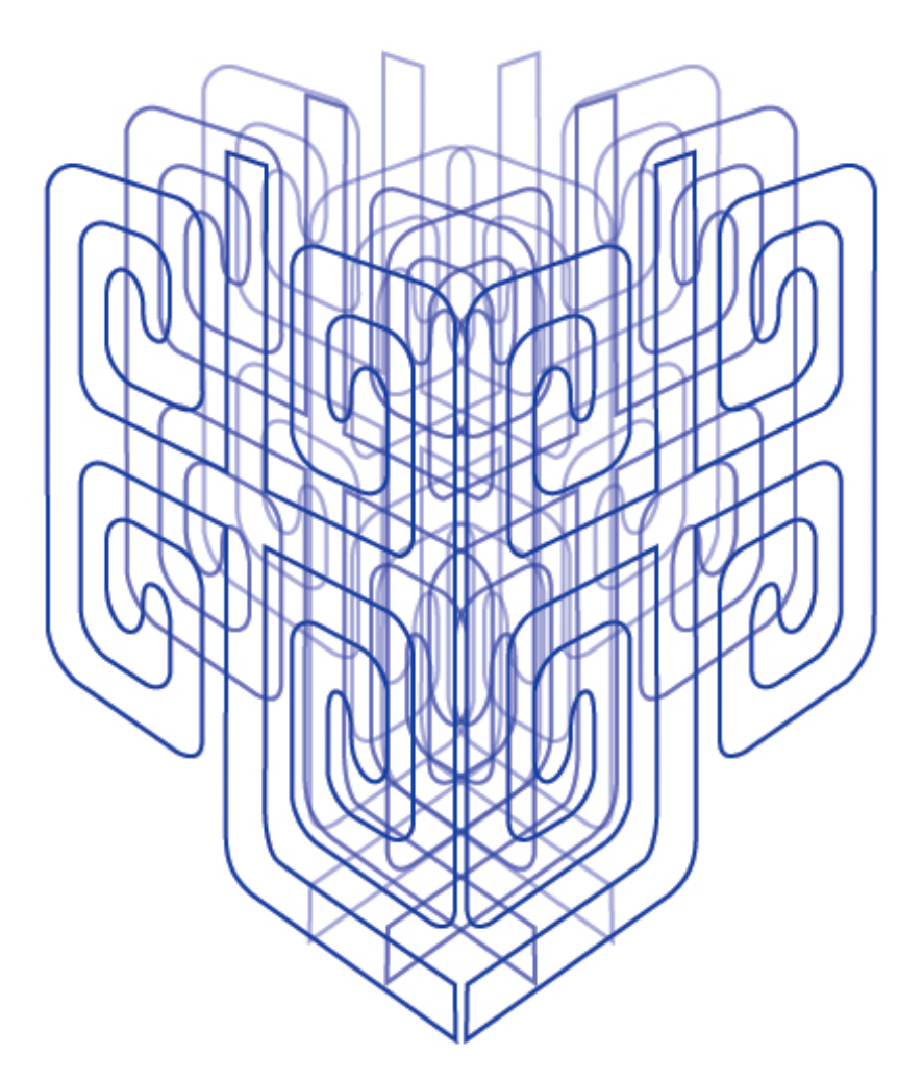
\includegraphics[trim=-680pt 0 0 -200pt,height=0.8\paperheight]{pic/njupt.pattern.pdf}
}
\begin{frame}
\frametitle{主要内容}
\tableofcontents
\end{frame}
\setbeamertemplate{background}{}
%------------------------------------------------------------

\section{模板用法}

\begin{frame}[fragile=singleslide]{latex与beamer}
  beamer 中每一页的内容都包含在frame环境中,这一部分将简单介绍beamer进行演示文稿制作的主要途径。
  本PPT内容均为拼凑而来,内容服务于展示beamer模板的需求,而不能保证正确性。

  个人建议,当重点关注其他内容时,可以采用“xelatex”一次编译,而需要编译完整文档时采用四次编译“xe->biber->xe->xe”。
  四次编译主要是为了参考文献的正确插入。

  可以使用”latexmk“来进行编译,其会自动调用相关工具进行编译,命令可以参考如下:

  \begin{verbatim}
    latexmk -xelatex main.tex
    latexmk -xelatex presentation.tex
  \end{verbatim}
\end{frame}

\begin{frame}[fragile=singleslide]{参考文献}
    虽然beamer官方不建议使用引用和脚注,但是由于答辩PPT主要用于演示研究成果,所以相关功能也加入到了文档中。
    参考文献的添加方式改为使用\textbf{biblatex},以下为我推荐的参考文献引用方式:

    在slides中使用脚注的形式来插入少量的参考文献,
    如使用\verb|\footfullcite{PRODEN}|其效果为\footfullcite{PRODEN}。

    在论文中,推荐比较像word中效果的命令,\verb|\cite{PRODEN}|用于句子后面引用,效果为“\cite{PRODEN}”。
    使用\verb|文献\parencite{PRODEN}|作为主语引用文献,效果为“文献\parencite{PRODEN}”

    附带脚注的插入方法为\verb|\footnote{xx}|效果为“\footnote{感谢南邮给予的学这些杂乱知识的机会} ”。

    详细参考文献引用的命令参见\textbf{biblatex}文档 \footnote{\url{https://ctan.org/pkg/biblatex}},
    或使用\verb|texdoc beamer|命令查看。
    
\end{frame}

\section{控制简介}

\begin{frame}{系统、控制、应用数学}
  控制理论是讲述系统控制科学中具有新观念、新思想的理论研究成果及其在各个领域中,特别是高科技领域中的应用研究成果,但是在民用领域即实际生活中有很严重的脱节。
\end{frame}

\begin{frame}{}
  \begin{enumerate}
    \item 经典控制理论:时域、频域的经典分析与设计(包括基于Nyquist、Bode图的方法,回路整形);根轨迹法;PID控制(Zieglar-Nichols);Wiener滤波;数字控制:Dalin控制,Smith控制,解耦控制,串级控制等;
    \item 现代控制理论:线性系统理论(状态空间法、代数理论、几何理论、多项式频率域方法);最优控制(变分法、极小值原理、动态规划、LQR等);最优状态估计(Kalman滤波、粒子滤波、无迹滤波等);系统辨识(经典与现代方法);自适应控制(模型参考自适应、自校正等);鲁棒控制(H-inf、u、棱边定理等);
    \item 非线性控制理论:非线性系统理论;滑膜变结构;Backstepping等;
  \end{enumerate}
\end{frame}

\begin{frame}{控制一瞥}
  \begin{figure}
    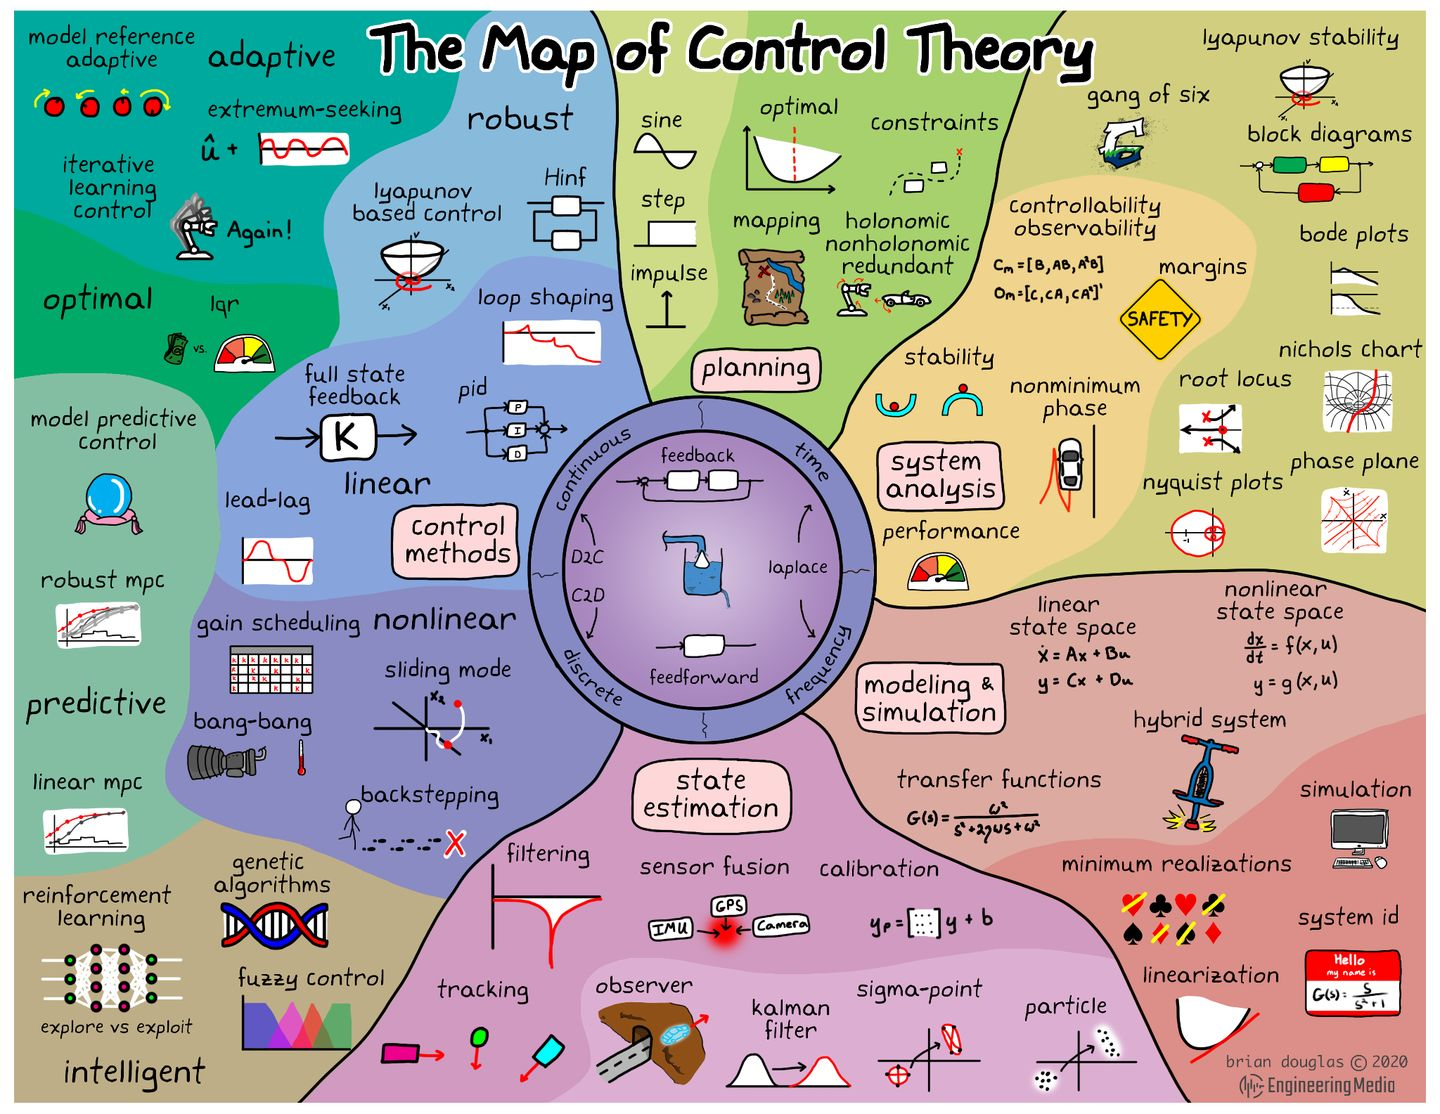
\includegraphics[width=0.8\textwidth]{pic/map_of_control.jpeg}
  \end{figure}
\end{frame}

\section{人工智能}

\begin{frame}{人工智能与控制}
  广义上来讲,机器学习跟控制理论本来就互相包含,比如强化学习(reinforcement learning)本身就起源于最优控制(optimal control),自适应控制(adaptive control)跟在线学习(online learning)以及在线优化(online optimization)息息相关,动态系统里的稳定性(stability)和鲁棒性(robustness)等概念也在机器学习里越来越重要。自动控制(automatic control)最大的目标就是赋予复杂系统“智慧”(full autonomy),这跟人工智能的目标是完全一致的。
\end{frame}

\section{总结与展望}
    \begin{frame}{控制的未来}
    \end{frame}



\section*{致谢}  
\setbeamertemplate{background} 
{
  \centering
  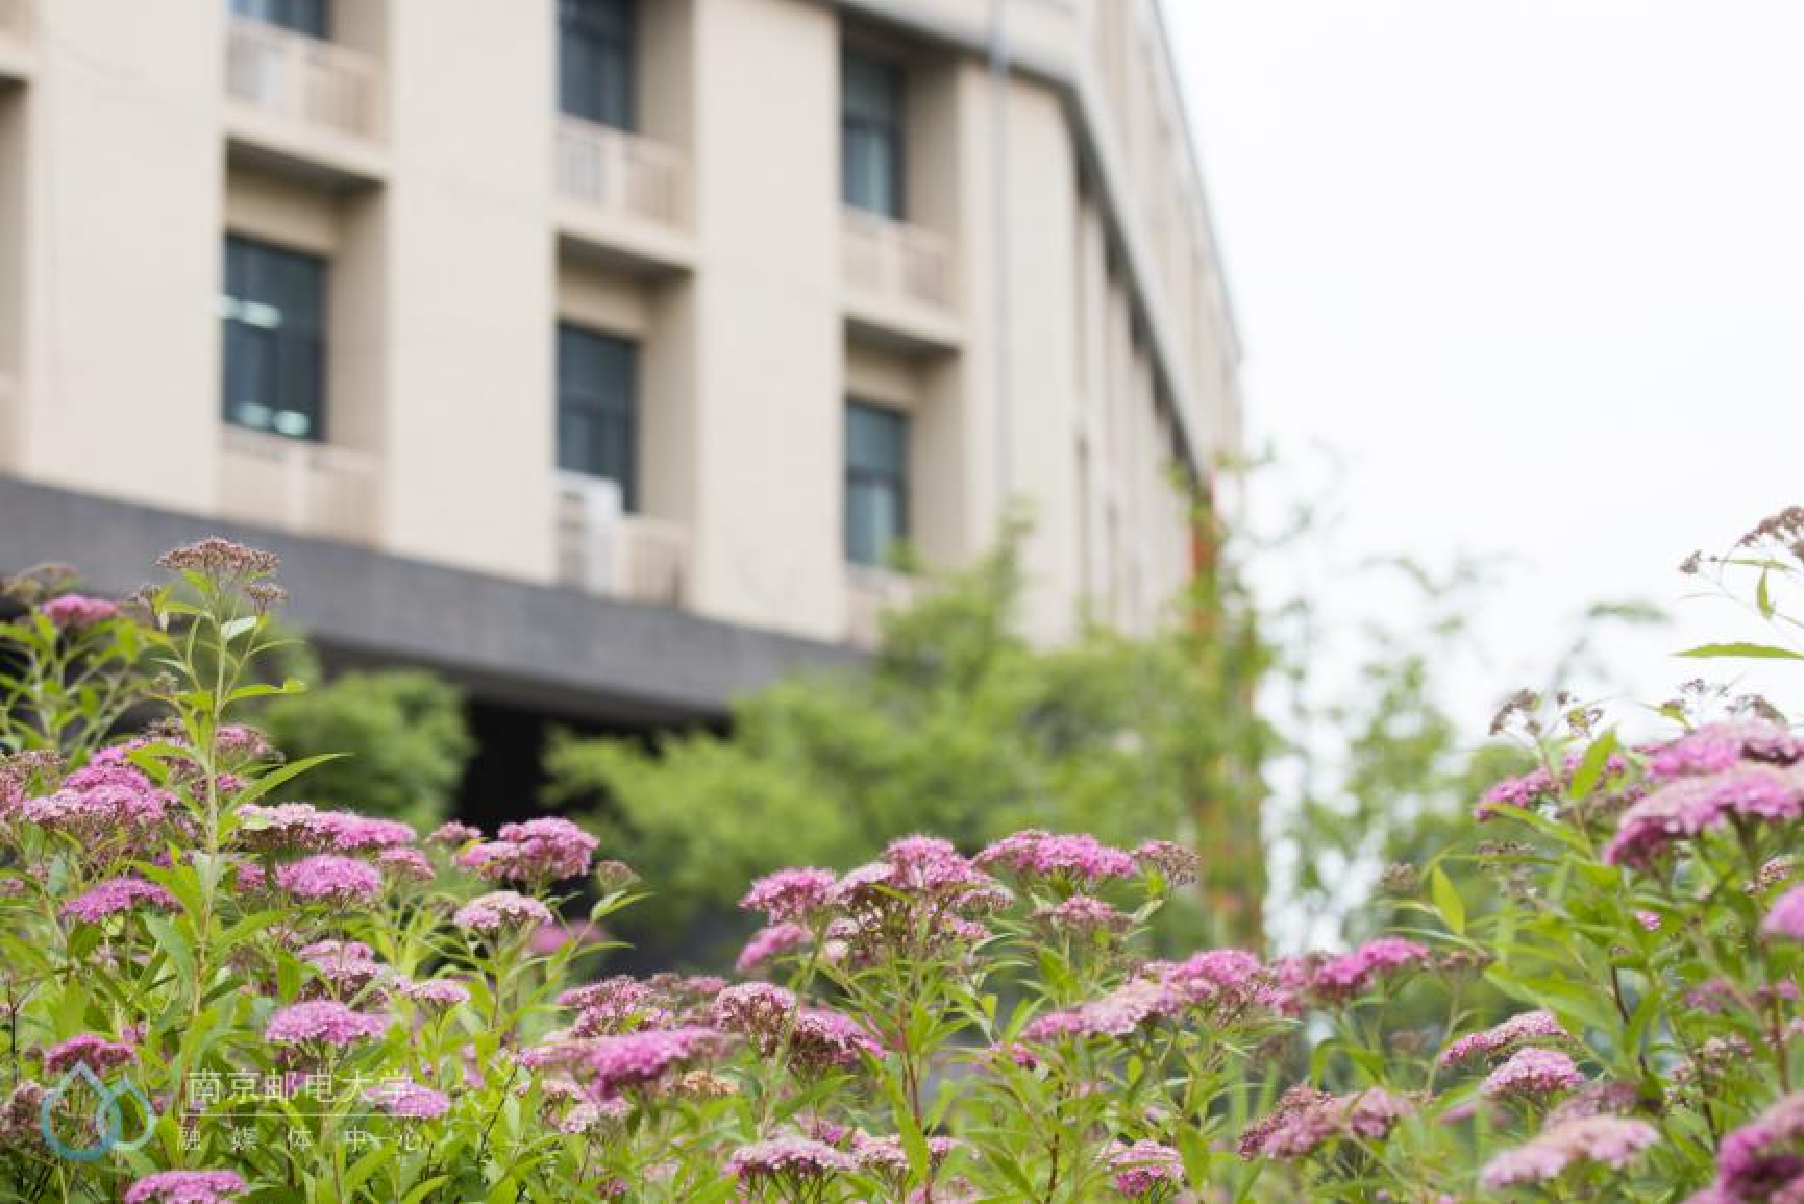
\includegraphics[trim=0 100 0 0,height=\paperheight,angle=0]{pic/njupt.flower.pdf}
}
\begin{frame}
\vfill
\centering
\begin{beamercolorbox}[sep=8pt,center,shadow=true,rounded=true]{title}
  \Huge{感谢聆听}
\end{beamercolorbox}
\vfill
\end{frame}
\setbeamertemplate{background}{}
\end{document}